% This file was created by matlab2tikz.
%
\documentclass[tikz]{standalone}
\usepackage[T1]{fontenc}
\usepackage[utf8]{inputenc}
\usepackage{pgfplots}
\usepackage{grffile}
\pgfplotsset{compat=newest}
\usetikzlibrary{plotmarks}
\usetikzlibrary{arrows.meta}
\usepgfplotslibrary{patchplots}
\usepackage{amsmath}

\newlength\figureHeight \setlength{\figureHeight}{6cm}
\newlength\figureWidth \setlength{\figureWidth}{10cm}
\begin{document}
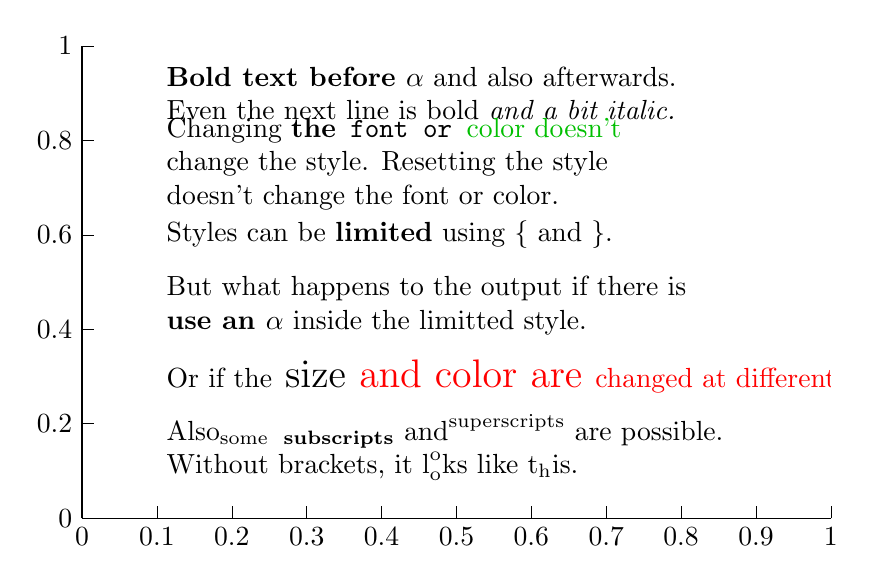
\begin{tikzpicture}

\begin{axis}[%
width=0.951\figureWidth,
height=\figureHeight,
at={(0\figureWidth,0\figureHeight)},
scale only axis,
every outer x axis line/.append style={black},
every x tick label/.append style={font=\color{black}},
every x tick/.append style={black},
xmin=   0,
xmax=   1,
every outer y axis line/.append style={black},
every y tick label/.append style={font=\color{black}},
every y tick/.append style={black},
ymin=   0,
ymax=   1,
axis background/.style={fill=white},
axis x line*=bottom,
axis y line*=left,
legend style={legend cell align=left, align=left, draw=black}
]
\node[right, align=left]
at (axis cs:0.1,0.9) {$\text{\bf{}Bold text before }\alpha\text{ and also afterwards.}$\\$\text{Even the next line is bold \it{}and a bit italic.}$};
\node[right, align=left]
at (axis cs:0.1,0.75) {$\text{Changing \bf{}the\ttfamily{} font or }\color[rgb]{0,0.75,0}\text{color doesn't}$\\$\text{change the style. Resetting \rm{}the style}$\\doesn't change the font or color.};
\node[right, align=left]
at (axis cs:0.1,0.6) {$\text{Styles can be }{\text{\bf{}limited}}\text{ using \{ and \}.}$};
\node[right, align=left]
at (axis cs:0.1,0.45) {But what happens to the output if there is\\${\text{\bf{}use an }\alpha\text{ inside}}\text{ the limitted style.}$};
\node[right, align=left]
at (axis cs:0.1,0.3) {$\text{Or if the}\fontsize{14}{0}\text{ size}\color{red}\text{ and color are }\fontsize{10}{0}\text{changed at different}\color{blue}\text{ points.}$};
\node[right, align=left]
at (axis cs:0.1,0.15) {$\text{Also}_{\text{some \bf{} subscripts}}\text{ and}^{\text{superscripts}}\text{ are possible.}$\\$\text{Without brackets, it l}^\text{o}_\text{o}\text{ks like t}_\text{h}\text{is.}$};
\end{axis}
\end{tikzpicture}%
\end{document}